\chapter{Etat de l'art}
\minitoc
\section{Introduction}
\section{Les modèles de consommation d'énergie DVFS et DPM}
L’énergie consommée par un processeur est l'integrale de
la puissance dissipée et du temps d’exécution. Nous utiliserons
principalement la notion de consommation énergétique et non de
puissance. Cette consommation énergétique est divisée en consommation
statique et consommation dynamique. Nous détaillons dans cette section
les modèles des consommations dynamique et statique et montrons que la
consommation statique est récemment devenue plus importante que la
consommation dynamique.
\subsection{Consommation dynamique}

Mei et al.\cite{Mei13}, ont défini la dissipation de puissance
dynamique par un circuit CMOS comme produit de Un coefficient constant
qui dépend de la technologie utilisée pour fabriquer la puce, par la
Carré de la tension et par la fréquence.
\begin{equation}
\pow_{dynamique} = \coeff * \freq * \volt^2 
\end{equation}
Où $\coeff$ correspond à la capacité de sortie du circuit et $\volt$ à
la tension d’alimentation.

Les solutions permettant de réduire la puissance dynamique dans les
circuits s’attachent par conséquent à réduire la fréquence de
fonctionnement. La relation précédente montre qu’il est moins
économique d’un point de vue énergétique de faire fonctionner un
circuit à pleine vitesse que de faire fonctionner un circuit à vitesse
réduite pendant un laps de temps plus important.

La technique permettant de réduire la vitesse du système est appelée
DVFS (Dynamic Voltage and Frequency Scaling) et tire parti du fait que
les processeurs ont plusieurs fréquences et plusieurs tensions de
fonctionnement. De nombreux algorithmes d’ordonnancement ont été
proposés utilisant cette solution \cite{WWDS94, YDS95, PS01}.
\subsection{Consommation statique}
La consommation statique des processeurs est en grande
partie due aux courants de fuite.  Dans un circuit idéal, cette
consommation statique est nulle mais, en réalité, un courant de fuite
existe et est responsable d’une consommation énergétique non
négligeable.  Ce courant de fuite provient du fait que les transistors
composant le circuit ne sont pas parfaits.  La consommation statique
peut être modélisée comme une constante \cite{KAB+03, SJPL08}.
Plusieurs solutions matérielles existent pour réduire la consommation
statique.  L’idée générale est d’éteindre une partie du circuit qui
n’est pas utilisée pour qu’aucun courant de fuite ne circule.  Cette
solution est appelée Power Gating. Dans les circuits actuels, les
puces peuvent être divisées en plusieurs parties, chaque partie ayant
la possibilité d’être éteinte indépendamment des autres parties du
circuit. Certaines sources \cite{HXW+10} affirme que l’énergie
statique représente jusqu’à 70\% de la consommation énergétique totale
dissipée par un processeur.  Plusieurs études confirment cette
affirmation \cite{Bor99, SBA+01, KAB+03, ABM+04, HSC+11, BBMB13}. Des
expériences ont également été faites \cite{SRH05, SPH05, LSH10} en
utilisant les algorithmes d’ordonnancement existants et les
conclusions de ces études est que réduire uniquement la consommation
dynamique peut entraîner une hausse de la consommation énergétique
globale car les composants sont actifs plus longtemps ce qui entraîne
une hausse de la consommation statique.

\section{Les états C-states du processeur}
\label{sec:cstate}
Pour réduire la consommation statique des processeurs, il est
nécessaire d’utiliser leurs états basse-consommation lors de leurs
périodes d’inactivité.  Nous appelons périodes d’inactivité les
périodes de temps durant lesquelles un processeur est inactif et où
aucune tâche n’est exécutée.  Les processeurs disposent maintenant de
plusieurs états basse-consommation où un certain nombre de composants
sont désactivés pour réduire la consommation énergétique.  Le problème
lié à l’utilisation de ces états basse-consommation est qu’éteindre,
rallumer ou changer d’état un processeur n’est pas anodin, que ce soit
du point de vue énergétique ou temporel. Nous définissons dans cette
section quatre notions relatives aux états basse-consommation. Nous
notons ns le nombre d’états basse-consommation de chaque processeur et
nous supposons que tous les processeurs possèdent les mêmes états
basse-consommation.

Consommation énergétique. Nous notons $Cons_s$ la consommation
énergétique de l’état basse-consommation s. C’est la consommation
énergétique dépensée lorsque le processeur se trouve dans cet état
basse-consommation.  Elle dépend du nombre de composants qui ont été
désactivés.  Plus ce nombre est important, plus la consommation
énergétique sera réduite.

Délai de transition. Nous définissons le délai de transition d’un état
basse-consommation comme le temps nécessaire pour revenir de cet état
basse-consommation à l’état actif.  C’est le temps nécessaire pour
réactiver tous les composants éteints durant l’état
basse-consommation.  Le délai de transition de l’état
basse-consommation s est noté $Del_s$.  Plus la consommation
énergétique de l’état basse-consommation est faible, plus son délai de
transition va être important car davantage de composants devront été
réactivés.

Pénalité énergétique. Nous notons $Pen_s$ la pénalité énergétique pour
revenir de l’état basse-consommation s à l’état actif.  Cette pénalité
énergétique correspond à la consommation énergétique nécessaire pour
réactiver tous les composants qui ont été éteints lors de l’activation
de l’état basse-consommation. Elle est consommée lorsque le processeur
passe de l’état basse-consommation à l’état actif, c’est-à-dire lors
du délai de transition. Plus la consommation énergétique d’un état
basse-consommation est faible, plus sa pénalité est importante.  nous
faisons l’hypothèse que l’évolution de la consommation énergétique
lors du réveil du processeur est linéaire. En supposant que la
consommation énergétique à l’état actif est de $Cons_{actif}$, la
pénalité énergétique d’un état basse-consommation est donc donnée par
la formule suivante :
\begin{equation}
Pen_s = \frac{1}{2} \times Del_s \times (Cons_{actif} - Cons_s)
\end{equation}
Nous faisons cette hypothèse car les pénalités énergétiques des états
basse-consommation sont difficiles à obtenir, les constructeurs ne
fournissant généralement que les valeurs des délais de transition pour
revenir des différents états basse-consommation (e.g. \cite{STM,
  MPC}). Néanmoins, nos contributions ne dépendent pas de cette
modélisation qui n’est utilisée que pour les évaluations et qui peut
être modifiée si les pénalités énergétiques des états
basse-consommation sont connues.

Break Even Time (BET). Nous définissons le BET comme la largeur
minimale de la pé-riode d’inactivité pour qu’il soit possible
d’activer un état basse-consommation \cite{AP11, CG06, DA08a}.  Chaque
état basse-consommation possède donc son propre BET et nous nommons
$BET$ le BET de l’état basse-consommation s.  Le BET de l’état
basse-consommation s correspond à la période de temps pour laquelle la
consommation énergétique du processeur à l’état actif est égale à la
consommation énergétique dans l’état basse-consommation s
(i.e. $Cons_s$) plus sa pénalité énergétique (i.e. $Pen_s$). Si la
longueur d’une période d’inactivité est inférieure au BET d’un état
basse-consommation donné, il est alors plus efficace énergétiquement de
laisser le processeur dans son état actif que d’activer l’état
basse-consommation en question. À noter que le BET ne permet pas de
savoir si une contrainte temps réel va être violée si cet état
basse-consommation est activé. C’est le délai de transition de l’état
basse-consommation qui importe alors pour réveiller à temps le
processeur.

Comme vu ci-dessus, nous faisons l’hypothèse que la consommation
énergétique évolue linéairement pour revenir de la consommation
énergétique d’un état basse-consommation à celle de l’état actif.
Avec cette hypothèse, le BET et le délai de transition d’un état
basse-consommation sont égaux.  En d’autre termes, il est toujours
plus efficace d’activer un état basse-consommation que de laisser le
processeur dans l’état actif si la longueur de la période d’inactivité
est supérieure au délai de transition d’un état basse-consommation. De
même que pour la pénalité énergétique, nous n’utilisons cette
hypothèse que dans nos évaluations et nos contributions séparent les
notions de BET et de délai de transition.  Exemples de processeurs

La majorité des processeurs actuels disposent de plusieurs fréquences
de fonctionnement et d’états basse-consommation pour réduire leur
consommation énergétique, nous en détaillons quelques-uns ici. Comme
notre objectif est de réduire la consommation statique, nous ne
détaillons pas les fréquences disponibles. Nous détaillons en revanche
les caractéristiques de chaque état basse-consommation, i.e. quels
sont les composants éteints et quelles sont les étapes requises pour
retrouver l’état actif.

Parmi les processeurs utilisés dans la littérature, citons le
Freescale MPC8536 \cite{MPC} utilisé par Awan et al. \cite{AP11, AP13,
  AYP13}. Ce processeur est basé sur une architecture PowerPC. Ses
états basse-consommation sont détaillés dans le Tableau 2.4.
\section{L'endormissement de processeur (Online VS Offline)}
\section{Le Modèle d'endormissement de Dsouza}
Anthony Rowe a proposé un algorithme d’ordonnancement appellé "Energy
Saving Rate Harmonized Scheduling (ES RHS)" \cite{Rowe10} basé sur la
période d’harmonisation qui améliore la consommation d’énergie pour
l’architecture multiprocesseur.  Dsouza l'a amelioré en proposant "ES
RHS+" dans cette section nous définirons la periode harmonique, puis
nous presenterons l'algorithme "Rate Harmonized Scheduling" et "Energy
Saving Rate-Harmonized Scheduling" enfin nous terminerons par
l'algorithme "Energy-Saving Rate-Harmonized Scheduling".

\subsection{Période d’harmonisation}

Soit un ensemble $\taskset{}$ de tache de $n$ taches périodiques
indépendantes, l’ensemble de tâche est ordonnée selon les périodes de
chaque tache de tel façon que $\period{1} \leq \period{2} \leq \cdots
\leq \period{n}$.  Un ensemble de taches $\{\task{1}, \task{2}, \dots,
\task{n} \}$ est harmonique si il existe un $\period{H}$ tel que
$\forall \task{i} / \frac{\period{i}}{\period{H}} \in \mathbb{Z}$

\subsection{Algorithme d’ordonnancement « Energy-Saving Rate-Harmonized Scheduling »}

En général RHS utilise un ensemble de Valeurs périodiques \{
$\period{H}^1,\period{H}^2,\dots ,\period{H}^3$ \} où $\period{H}^i
\leq \period{i}$ pour $i \in \{1, \cdots, n \}$, Et les valeurs sont
harmoniques. Les périodes harmoniques sont appelées "périodes de base
harmonisées", Et toute les taches ont le même temps de reveil de
$\task{1}$ = $r_1$ = 0.

Les tâches $\{\task{1}, \task{2}, \cdots, \task{n} \}$ dans l’ensemble
tâches donné sont réveillées selon leurs arrivée comme dans le modèle
classique Toutefois, chaque job de $\task{i}$ ne peut être exécutée
que à sa prochaine frontière périodique la plus proche de
$\period{H}^i$ \cite{Rowe10}.

Dans le L’ordonnancement RHS de base, \{ $\period{H}^1 = \period{H}^2
= … = \period{H}^n = \period{H}$ \}, $\period{H}$ Est simplement
appelé période d'harmonisation et $\period{H} \leq \period{1}$. Les
tâches qui arrivent avant ou après les multiples entiers de
$\period{H}$ ne sont pas autorisée à s'exécuter jusqu'à la prochaine
limite la plus proche de quand ils sont lancés en fonction de leur
priorité (voir figure). Les tâches qui ne sont pas admissibles sont
retardées jusqu'à la prochaine limite.

$\period{H}$ est choisi de manière à améliorer l'ordonnancement
\cite{Rowe10}. Supposer $\Psi=\{\task{j} /
\period{j}~<~2\period{1},~j~\neq 1\}$. si $\Psi = \emptyset,
\period{H} = \period{1}.~sinon~\period{H} = \frac{\period{1}}{2}$.

\begin{theoreme}[\cite{Rowe10}]
un ensmeble de taches $\taskset{}$ est faisable sous RHS si $U \leq
0.5$.
\end{theoreme}

\begin{theoreme}
le calcul du pire temps de reponse $\resp{i}{}$ [23,24] dans le cas de RHS
peut etre redéfini comme suit : \\
%\begin{equation}
\begin{align}
r_{i,0} & = \charge{i} + \period{H} 
\\ r_{i,k+1} & = \charge{i} + \period{H} + \sum_{j = 1}^{i-1} \bigg \lceil \frac{\resp{i}{k}}{\period{j}}\bigg \rceil \charge{j}
\end{align}
%\end{equation}
\end{theoreme}

\begin{theoreme}[\cite{Rowe10}]
Soit $\taskset{} = \{\task{1}, \task{2}, \dots, \task{n} \}$ un
ensemble de tache periodiques indépendantes.

Si il existe une tache $\task{i}$ avec un pire temps de reponse
$\resp{i}{}$ tel que $r_i > \deadline{i}$ alors l'ensemble de tache
$\taskset{}$ est non ordonnançable.
\end{theoreme}

\subsection{Energy-Saving Rate-Harmonized Scheduling}

comme vu dans la section \ref{sec:cstate}, les processeurs sont dotés
de mode de basse consommation.  par exemple: un processeur
"power-aware" a :
\begin{itemize}
\item mode actif avec une consommation d'énergie $PW_{active}$
\item mode sommeil avec une consommation d'énergie
  $PW_{idle}$ et un temps de bascule $ST_{idle}$
\item mode sommeil profond avec une consommation d'énergie
  $PW_{sleep}$ et un temps de bascule $ST_{sleep}$
\end{itemize}
avec $PW_{active} > PW_{idle} \gg PW_{sleep} $ et $ ST_{idle} \ll
ST_{sleep}$.

Quand il n'y a aucune tache préte à s'executer, le processeur et
generalement en mode sommeil, cependant si il y a une tache qui arrive
avant $\S\period{sleep}$ unité de temps,il ne peut passer en mode
sommeil.

ES-RHS présente une propriété intéressante, où tous les periode de
sommeil précède et est contiguë au sommeil profond durée peuvent
toujours être fusionnée [10]. Par conséquent, en harmonisant les
exécutions de tâches non harmoniques, ES-RHS peut produire des periode
de sommeil optimal. D'souza \cite{DAR16} a redéfini la notion
d'harmonisation pour ameliorer l'ordonnancemen ES-RHS.
\subsection{Energy-Saving Rate-Harmonized Scheduling+}
\indent Une tâche est susceptible d'être exécutée lorsque le
processeur est occupé ou une limite de la période d'harmonisation a
été atteinte. Cette redéfinition permet aux taches d'etre préte à
s'executer plus tôt par rapport à l'ordonnanceur de ES-RHS
\cite{Rowe10}.

La table \ref{tab:exempleRHS} et les figures \ref{fig:exempleRHS} et
\ref{fig:exempleRHS+} illustrent la difference entre les deux
ordonnanceur et l'apport de D'souza.

\begin{table}[h]
\begin{center}
\begin{tabular}{|c|c|c|}
 \hline$\task{i}$ & $\charge{i}$ & $\period{i}$ \\ 
 \hline1 & 1 & 10 \\ 
 \hline 2 & 4 & 23 \\ 
 \hline 3 & 3 & 36 \\ 
 \hline 
 \end{tabular}
\end{center}
\caption{Ensemble de taches} \label{tab:exempleRHS}
\end{table}

\begin{center}
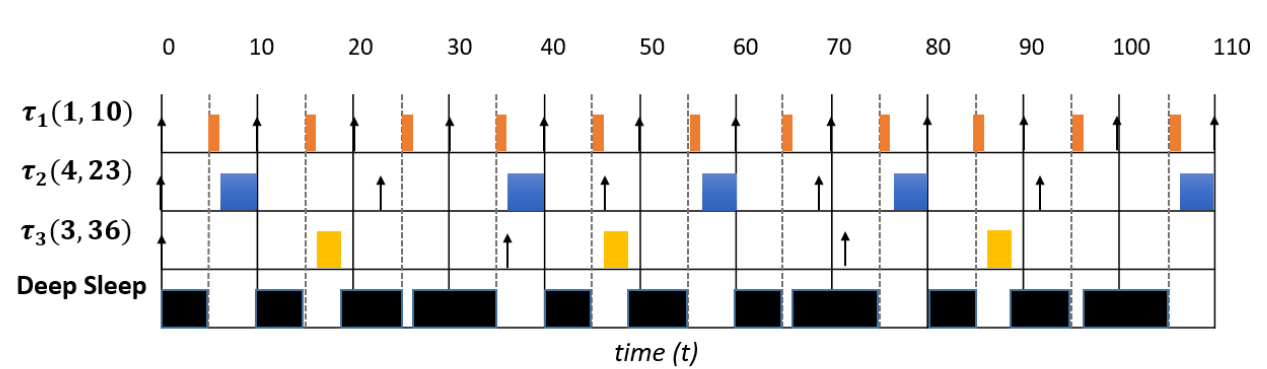
\includegraphics[height=4cm,width=12cm]{part1/rhs.png}
\captionof{figure}{Energy-Saving RHS}
\label{fig:exempleRHS}
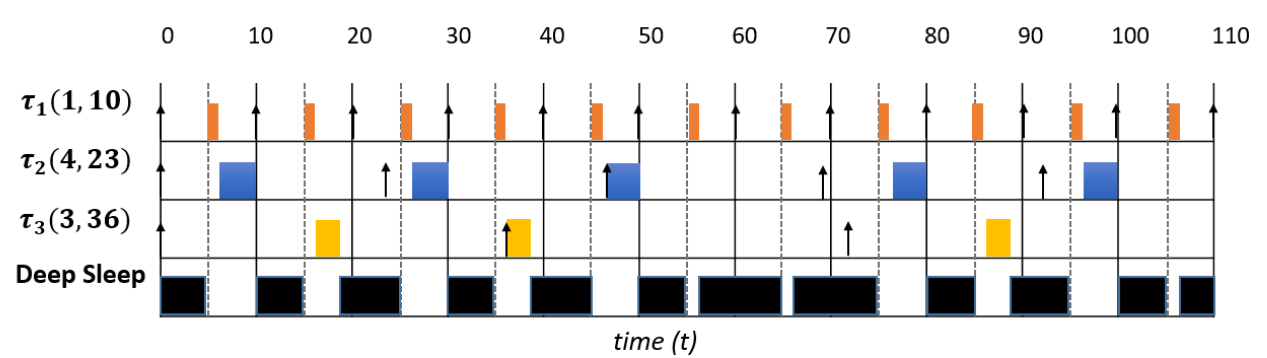
\includegraphics[height=4cm,width=12cm]{part1/rhs+.png}
\captionof{figure}{Energy-Saving RHS+}
\label{fig:exempleRHS+}
\end{center}

\section{Conclusion}
